\documentclass{article}
\usepackage{graphicx}
\usepackage[utf8]{inputenc}
\usepackage{fullpage}
\usepackage{listings}
\usepackage{xcolor}
\usepackage{url}
\usepackage[linesnumbered,ruled,vlined]{algorithm2e}
\usepackage{enumitem}

\usepackage{amsmath}
\usepackage{amsfonts}
\usepackage{amssymb}

\parindent0in
\pagestyle{plain}
\thispagestyle{plain}

\newcommand{\assignment}{Homework 1}
\newcommand{\duedate}{July 19, 2019}

% \renewcommand\thesubsection{\arabic{subsection}}

\title{Homework 1}
\date{}

\begin{document}
	
	Fundação Getulio Vargas\hfill\\
	Estruturas de Dados e Algoritmos\hfill\textbf{\assignment}\\
	Aluno: Marcelo Bianchi Barata Ribeiro\\
	Prof.\ Jorge Poco\hfill\textbf{Due:}: \duedate\\
	\smallskip\hrule\bigskip
	
	{\let\newpage\relax\maketitle}
	\maketitle
	
	
	\section{Induction [3pts]}
	Answers should be written in this document. 
	
	\begin{enumerate}
		\item Prove by Induction that:
		\( \sum_{i=1}^{n}i^2=\frac{n(n+1)(2n+1)}{6} \qquad\forall n \geq 0\)
		
		\textbf{Resposta}: No caso base, n = 1, a fórmula é valida, dado que \( \sum_{i=1}^{1}i^2=1 = \frac{1(2)(3)}{6} \)
		
		Suponhamos que ela valha para um certo n, ou seja, 
		\( 1^2+2^2+3^2+...+n^2 = \frac{n(n+1)(2n+1)}{6} \)
		
		Somando (n + 1) a ambos os lados da igualdade, obtemos:
		
		\( 1^2+2^2+3^2+...+n^2+(n+1)^2 = \frac{n(n+1)(2n+1)}{6}+(n+1)^2 =  \frac{(n+1)(2n^2+n) + (n+1)(6n+6)}{6} = \frac{(n+1)(2n^2+n+6n+6)}{6} = \frac{(n+1)(2n^2+7n+6)}{6} = \frac{(n+1)(n+2)(2n+3)}{6}\)
		
		\item Prove by Induction that:
		$\forall n \geq 7$ it is true $3^n<n!$
		
		\textbf{Resposta}: No caso base, n = 7, a fórmula é valida, dado que $3^7 = 2187 < 5040= 7!$
		
		Suponhamos que ela valha para um certo n, ou seja, 
		$3^n<n!$
		
		Multiplicando ambos os membros da igualdade por 3, obtemos: \(3^{(n+1)}<3n!\)
		Mas, para todo $n \geq 7$, temos que $(n+1)! > 3n!$. Portanto, $3^{(n+1)}<(n+1)!$, o
		que mostra que a desigualdade também vale para n+1. Logo, por inducão, a desigualdade vale para todo $n \geq 7$.
		
		\item Prove by Induction that $\forall n \geq 0$
		\[
		\left \lceil\frac{n}{2} \right \rceil=
		\left\{
		\begin{array}{ll}
		\frac{n}{2}& \textrm{si $n$ es par}\\
		\frac{n+1}{2}& \textrm{si $n$ es impar}
		\end{array}
		\right.
		\]
		\textbf{Resposta}: No caso base, n = 0 (par) ou n = 1 (ímpar), a fórmula é valida, dado que:
		
		$\lceil\frac{0}{2} \rceil= 0 = \frac{n}{2}$
		
		$\lceil\frac{1}{2} \rceil= 1 = \frac{n+1}{2}$
		
		Podemos resolver agora considerando n = 2m se n for par e n = 2m+1 se n for ímpar. Logo: para n par: $\lceil\frac{n}{2} \rceil= \lceil\frac{2m}{2} \rceil= \lceil m \rceil = m = \frac{n}{2}$
		
		Para n ímpar: $\lceil\frac{n}{2} \rceil= \lceil\frac{2m+1}{2} \rceil= \lceil m+\frac{1}{2} \rceil = m + 1= \frac{2m+2}{2} = \frac{(2m+1)+1}{2} = \frac{n+1}{2}$
		
		Logo, por indução, a proposição é válida.
		
		\item Prove by induction that a number is divisible by 3 if and only if the sum of its digits is divisible by 3.
		
		\textbf{Resposta}: No caso base, 3, 6 e 9 são divisíveis por 3. O primeiro múltiplo de dois dígitos, 12, também é. Além disso, 1 + 2 = 3, ou seja, a soma dos dígitos é divisível por 3.
		
		Suponhamos que a afirmação seja válida para um certo n com m dígitos, sendo n = $i_{1}*10^n+i_{2}*10^{n-1}+...+i_{m}*10^{0}$
		
		Sabemos que 10\%3=1. Portanto, o resto da divisão da soma dos dígitos por 3 pode ser escrita como $i_{1}*1^n+i_{2}*1^{n-1}+...+i_{m}*1^{0} = i_{1}+i_{2}+...+i_{m}$
		Ou seja, dado a igualdade anterior, a soma dos dígitos de n é divisível por 3 se e somente se n\%3=0.
		
		Seguindo a sequência, (n+3)\%3=0. Somando 3 na soma dos dígitos, temos $i_{1}+i_{2}+...+i_{m} + 3$. Como $(i_{1}+i_{2}+...+i_{m})\%3 = 0$ e 3\%3=0, temos que a soma dos dígitos de n+3 também é divisível por 0.
		
		\item Prove that any integer greater than 59 can be formed using only 7 and 11 cent coins.
		
		\textbf{Resposta}: Tal tipo de questão é conhecido como problema da moeda de Frobenius. Refraseando, para todo $n>59$, existe x,y tal que 7x+11y = n
		
		No caso base, a fórmula é válida, pois 60 = 7*7 + 11*1.
		
		Suponhamos que ela valha para um certo n, ou seja, 7x+11y = n
		
		Para o caso n+1, basta encontrar 7x'+11y'=n+1
		Fazendo, x' = x-3 e y' = y+2, temos 7(x-3)+11(y+2) = 7x+11y-21+22 = 7x+11y+1 = n+1
		
		Portanto, por indução, a proposição é válida.
		
		\item Prove by induction that $F_{n+k}=F_{k}F_{n+1}+F_{k-1}F_{n}$
		
		\textbf{Resposta}: no caso base, n = 1, temos que $F_{k+1}=F_{k}F_{2}+F_{k-1}F_{1}$. Como $F_{1} = 1, F_{2} = 1$, temos que $F_{k+1}=F_{k}+F_{k-1}$, comprovando a validade do caso base.
		
		Suponhamos que ela valha para um certo n, precisamos provar para $F_{n+k+1}$, que é o mesmo que $F_{n+k} + F_{n+k-1}$. Somando $F_{n+k-1}$ ao outro lado da igualdade, temos:\\ 
		$F_{n+k+1}=F_{k}F_{n+1}+F_{k-1}F_{n}+F_{n+k-1}$ (1)\\
		Agora, como $F_{n+k-1} = F_{k}F_{n}+F_{k-1}F_{n-1}$, usando isso em (1), temos que: \\ $F_{n+k+1}=F_{k}F_{n+1}+F_{k-1}F_{n}+F_{k}F_{n}+F_{k-1}F_{n-1} = \\
		F_{k}(F_{n+1}+F_{n})+F_{k-1}(F_{n}+F_{n-1}) = \\
		F_{k}F_{n+2}+F_{k-1}F_{n+1}$ \\
		Portanto, por indução, a proposição é válida.
		
		\item Prove by induction in $n$ that \(\sum_{m=0}^{n}{n \choose m}=2^n\)
		
		\textbf{Resposta}: No caso base, n=0, a fórmula é válida, dado que \(\sum_{m=0}^{0}{0 \choose 0}=1=2^0\)
		
		Suponhamos que ela valha para um certo n, ou seja, \(\sum_{m=0}^{n}{n \choose m}=2^n\)
		
		Consideramos a convenção de que 
		${n \choose m} = 0$ se 
		$m \notin \{0,1,...,n\}$. Sabemos também que a sucessão de coeficientes binomiais satisfaz a seguinte relação de recursão: 
		\({n \choose m} = {n-1 \choose m} + {n-1 \choose m-1}\)
		
		Com a inclusão de n+1 no somatório, temos: 
		\(\sum_{m=0}^{n+1}{n+1 \choose m} = \sum_{m=0}^{}[{n \choose m} + {n \choose m-1}] = \sum_{m=0}^{}{n \choose m} + \sum_{m=0}^{}{n \choose m-1} = 2^n + 2^n = 2^n*2 = 2^{(n+1)}\)
		
		Portanto, por indução, a proposição é válida.
		
		\item Prove by induction that a graph with $n$ vertices can have at most  $\frac{n(n-1)}{2}$ edges.
		
		\textbf{Resposta}: 
		No caso base, n=1, a fórmula é válida, dado que $\frac{1(1-1)}{2} = 0$
		
		Suponhamos que ela valha para um certo n, ou seja, número máximo de arestas =  
		$\frac{n(n-1)}{2}$
		
		Sabemos que a cada novo vértice, o máximo de novas conexões ocorre ao se conectar com todos os vértices anteriores, ou seja, para n+1 vértices, adiciona-se n arestas no máximo.
		
		Com isso, obtemos: $\frac{n(n-1)}{2} + n = \frac{n^2 - n + 2n}{2} = \frac{n^2 + n}{2} = \frac{(n+1)n}{2}$. 
		
		Portanto, por indução, a proposição é válida.
		
		
		\item Prove by induction that a complete binary tree\footnote{http://web.cecs.pdx.edu/~sheard/course/Cs163/Doc/FullvsComplete.html} with $n$ levels has $2^n-1$ vertices.
		
		\textbf{Resposta}: 
		No caso base, n=1, a fórmula é válida, dado que $2^1-1 = 1$
		
		Suponhamos que ela valha para um certo n, ou seja, número de vértices =  
		$2^n-1$
		
		Sabemos que, sendo a árvore binária completa, com acréscimo do nível n, adiciona-se $2^{(n-1)}$ vértices.
		
		Com isso, com a adição do nível n+1, temos: $2^n-1 + 2^n = 2^n*2-1 = 2^{(n+1)}-1  $ 
		
		Portanto, por indução, a proposição é válida.
		
		\item A polygon is convex if each pair of points in the polygon can be joined by a straight line that does not leave the polygon. Prove by induction in $n>3$ that the sum of the angles of a polygon of $n$ vertices is $180(n-2)$.
		
		\textbf{Resposta}: No caso base, n=4, a proposição é válida, dado que 180*2 = 360 = soma dos ângulos de um quadrado.
		
		Suponhamos que ela valha para um certo n, ou seja, soma dos ângulos de um polígono = $180(n-2)$
		
		Sabemos que um polígono permite o desenho de n-2 triângulos internos e que a adição de um novo vértice permite o acréscimo de um novo triângulo. Sabemos também a soma dos ângulos de um triângulo = 180. Com isso, para n+1 vértices, adicionamos 180 à soma de ângulos. Logo, $180(n-2) + 180 = 180n - 360 + 180 = 180((n+1)-2)$
		
		Portanto, por indução, a proposição é válida.
		
	\end{enumerate}
	
	\section{Correctness of bubblesort [2pts]}
	Bubblesort is a popular, but inefficient, sorting algorithm. It works by repeatedly swapping adjacent elements that are out of order.
	
	\begin{algorithm}[H]
		\SetAlgoLined
		\For{$i = 1$ \textbf{to} $A.length -1$} {
			\For{$j = A.length$ \textbf{downto} $i + 1$} {
				\If{$A[j] < A[j-1]$} {
					exchange $A[j]$ with $A[j-1]$
				}
			}
		}
		\caption{BUBBLESORT(A)}
	\end{algorithm}
	
	\begin{enumerate}[label=\Alph*]
		\item Let $A'$ denote the output of BUBBLESORT(A). To prove that BUBBLESORT is correct, we need to prove that it terminates and that
		
		\begin{equation} \label{eq:1}
		A'[1] \leq A'[2] \leq ... \leq A'[n]
		\end{equation}
		
		where $n = A.length$. In order to show that BUBBLESORT actually sorts, what else do we need to prove?
		
		Precisamos também provar que A' possui os mesmos elementos que A, mas não necessariamente na mesma ordem.
		
		The next two parts will prove inequality~(\ref{eq:1}).
		
		\item State precisely a loop invariant for the \textbf{for} loop in lines 2–6, and prove that this loop invariant holds. Your proof should use the structure of the loop invariant proof presented in this chapter.
		
		Tal como indicado no livro "Introduction to Algorithms", de Thomas Cormen, para provar que o loop de um algoritmo cumpre sua função, devemos demostrar que as três condições de um loop invariant são satisfeitas:
		\begin{itemize}
			\item Inicialização: é verdadeiro antes da primeira iteração do loop.
			\item Manutenção: é verdadeiro tanto antes da iteração atual do loop, quando antes da iteração seguinte. 
			\item Finalização (já mencionado no enunciado): ao final, a invariante nos dá uma propriedade que ajuda a demonstrar que o algoritmo está correto.
		\end{itemize}
		
		Os dois primeiros argumentos são semelhantes ao de prova por indução. O terceiro interrompe o processo.
		
		Na sublista A[j...], A[j] é o menor dos elementos
		
		\begin{itemize}
			\item Inicialização: Trivial, pois A[j...] é constituído por um único elemento, o último da lista, antes da primeira iteração do loop.
			\item Manutenção: A cada iteração, se $A[j-1] < A[j]$, faz-se a troca dos elementos, tornando A[j-1] o menor entre os dois. Tal processo continua até que j = i+1, o que encerra o loop interno. A cada ativação desse loop, garante-se que na lista A[j...], A[j] será o menor dos elementos.
			\item Finalização: Ao final, quando j=i, garantimos que A[i] é o menor elemento da sublista A[i...].
		\end{itemize}
		
		\item Using the termination condition of the loop invariant proved in part (B), state a loop invariant for the for loop in lines 1–7 that will allow you to prove inequality~(\ref{eq:1}). Your proof should use the structure of the loop invariant proof presented in this chapter.
		
		A sublista A[1,...,i] possui elementos ordenados em ordem crescente.
		
		\begin{itemize}
			\item Inicialização: Antes da primeira iteração, temos apenas um elemento e a sublista é claramente ordenada.
			
			\item Manutenção: O loop interno assegura que a cada iteração, A[i] será o menor elemento da sublista A[i...]. Com isso, garante-se que a cada iteração, sendo os elementos i,k $\in A[1,...,i], A[i]<A[k], \forall i<k$
			
			\item Finalização: O loop é encerrado quando i chega ao final da lista, ou seja, i=n, sendo n = A.length. A sublista final A[i,...,n] possui todos os seus elementos ordenados.
		\end{itemize}
		
		\item What is the worst-case running time of BUBBLESORT? How does it compare to the running time of insertion sort?
		
		No pior caso, quando os elementos estão ordenados em ordem decrescente, o running time de bubble sort é $\Theta (n^2)$
		Quanto ao algoritmo insertion sort, no pior caso, o running time também é $\Theta(n^2)$
		
		Por outro lado, o melhor caso de insertion sort é $\Theta(n)$, enquanto que o melhor caso de bubble sort continua sendo $\Theta(n^2)$
		
	\end{enumerate}
	
	
	\section{Growth of Functions [2pts]}
	
	\begin{enumerate}[label=\Alph*]
		\item For each of the following pairs of functions, either $f(n)$ is in $O(g(n))$, $f(n)$ is in $\Omega(g(n))$, or $f(n) = \Theta(g(n))$. Determine which relationship is correct and briefly explain why.
		
		Lembrando que: 
		\begin{itemize}
			\item f(n) = O(g(n)) se $\exists n_{0}\in \mathbb{N}, c \in \mathbb{R}_+$ tal que $\forall n \in \mathbb{N}, n\geq n_{0} \to f(n) \leq cg(n)$
			\item $f(n) = \Omega(g(n))$ se $\exists n_{0}\in \mathbb{N}, c \in \mathbb{R}_+ $ tal que $\forall n \in \mathbb{N}, n\geq n_{0} \to f(n) \geq cg(n)$
			\item $f(n) = \Theta(g(n))$ se f(n) = O(n) e f(n) = $\Omega(g(n))$
			\\ \\
			Resolvendo as questões:
		\end{itemize}
		\begin{itemize}
			\item $f(n) = \log n^2$; $g(n) = \log n + 5$ \\
			f(n) = $\Theta (g(n))$, pois f(n) = O(n) e f(n) = $\Omega(g(n))$ \\
			f(n) = $O(g(n))$, pois usando c = 3 e $n_0$ = 1, temos $f(n) = 2\log n \leq 3\log n  + 15 = cg(n)$\\
			f(n) = $\Omega(g(n))$, pois usando c = 1 e $n_0$ = 32, temos $f(n) = 2\log n \geq \log n  + 5 = cg(n)$
			
			\item $f(n) = \log^2 n$; $g(n) = \log n$ \\
			f(n) = $\Omega(g(n))$, pois usando c = 1 e $n_0$ = 4, temos $f(n) = \log n\log n = 4 \geq 2 = \log n = cg(n)$
			
			\item $f(n) = n\log n + n$; $g(n) = \log n$ \\
			f(n) = $\Omega(g(n))$, pois usando c = 1 e $n_0$ = 2, temos $f(n) = n\log n + n = 4 \geq 1 = \log n = cg(n)$
			
			\item $f(n) = 2^n$; $g(n) = 10n^2$ \\
			f(n) = $\Omega (g(n))$, pois usando c = $\frac{1}{10}$ e $n_0$ = 5, temos $f(n) = 2^n = 32 \geq 25 = n^2 = cg(n)$
		\end{itemize}
		
		\item Prove that $n^3 -3n^2 -n+1 = \Theta(n^3)$. \\
		$n^3 -3n^2 -n+1 = O(n^3)$, pois usando $c = 6, n_0 = 1$, temos $ n^3 -3n^2 -n+1 \leq n^3 +3n^3 +n^3+n^3  = 6n^3 $
		
		$n^3 -3n^2 -n+1 = \Omega(n^3)$, pois usando $c = \frac{1}{10}, n_0 = 5$, temos $ 5^3 -3*5^2 -5+1 = 46 \geq 12.5 = \frac{5^3}{10} $
		
		\item Prove that $n^2 = O(2^n)$. \\
		Precisamos encontrar c e $n_0$ tal que $f(n) \leq cg(n) \forall n > n_0$. Usando $c = 1, n_0 = 5$, temos $ 5^2 = 25 \leq 32 = 2^5$
		
	\end{enumerate}
	
	
	\section{Insertion Sort - Mergesort - Quicksort [3pts]}
	Implement the insertion sort, merge sort and quicksort using the template \texttt{test.py} (use Python 3.X). Create a \texttt{test.cpp} file and write the equivalent code from \texttt{test.py} in C++, ie., the functions: main, \texttt{insertion\_sort}, \texttt{merge\_sort}, \texttt{quicksort} and \texttt{is\_sorted}. For the random number generations you can use the \texttt{rand} function from \texttt{cstdlib}\footnote{\url{http://www.cplusplus.com/reference/cstdlib/rand/}}. Your code should print the tuple (number of objects, time insertion\_sort, time merge\_sort, time quicksort)
	
	You must submit both \texttt{test.py} and \texttt{test.cpp}. Graphs and descriptions must be included in this document. 
	
	\subsection{Random Order}
	\begin{enumerate}
		\item Create 10 sets of numbers in random order. The sets must have \{10k, 20k, 30k, ..., 100k\} numbers.
		
		Fiz com 10 sets indo de 270 a 2.700, pois o python limitava a quantidade máxima de resursões, principalmente no quicksort. No C++ consegui trabalhar com até 100.000 valores, mas eu não teria como comparar com python.
		
		\item Sort these numbers using the 3 algorithms and calculate the time each algorithm takes for each set of numbers.
		
		Ver códigos.
		
		\item Generate a plot (using excel or another tool) showing a \emph{linechart}, where the $x$-axis is the ``number of elements", and the $y$-axis is the time that the algorithms took in C++ and Python. This plot must have 6 lines of different colors with a legend.
		
		IMAGENS FORAM ALOCADAS AO FINAL DO DOCUMENTO, NA SEÇÃO IMAGENS.
		
		\item Write a small paragraph (3 to 4 lines) describing the results.
		
		Obs: criei gráficos com os 6 algoritmos e também com apenas C++ para termos de comparação, dado que os algoritmos de python suprimiam os de C++.\\
		Em 1º lugar, vemos claramente que o tempo de execução com python é muito maior do que em C++, o que faz sentido, devido à forma como as duas linguagens de programação funcionam. Também vemos claramente que a eficiência dos algoritmos segue conforme a notação Big-O. 
		Insertion sort é o menos eficiente $[O(n^2)$ em geral, o que fica evidente no gráfico. Mergesort é sempre O(nlogn). Quicksort é em média O(nlogn).
		
	\end{enumerate}
	
	\subsection{Ascending Order}
	
	
	
	Nesse caso, insertion sort é o mais eficiente, quando já está ordenado na ordem correta [O(n)]. Quicksort continua igual apenas se a escolha do pivô for aleatória. Se eu tivesse escolhido o pivô como o último elemento, estaria no pior dos casos (quando está ordenado) $[O(n^2)$, pois o algoritmo está sempre tentando separar a lista pegando o último elemento das listas como pivô. No gráfico comente com C++, mergesort continua igual e segue junto com quicksort. No python isso não acontece por causa de alguma configuração do algoritmo.
	
	\subsection{Descending Order}
	
	
	Nesse caso, insertion sort é o pior, quando está ordenado ao contrário do que desejamos $[O(n^2)$. Quicksort continua igual a antes, dado a escolha aleatória do pivô. Mergesort continua igual.
	
	\subsection{Imagens}
	\begin{figure}[!h]
		\centering
		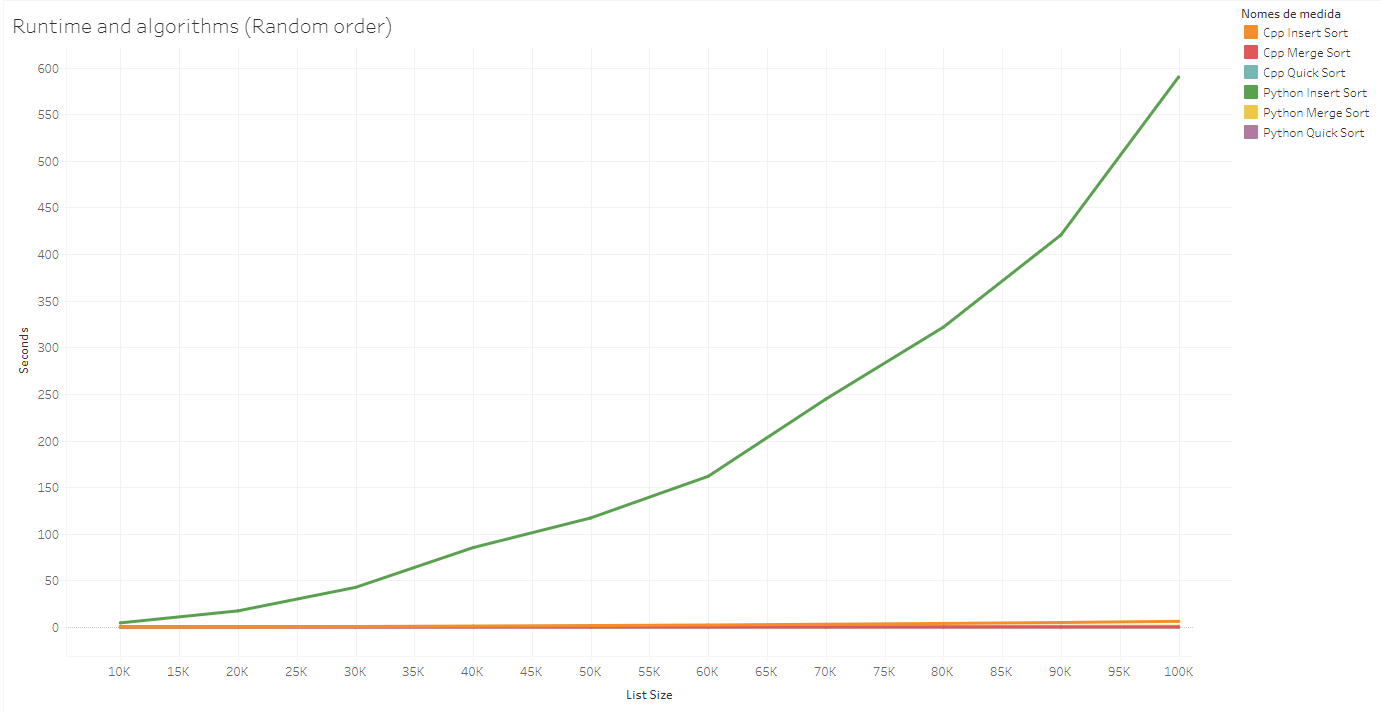
\includegraphics[scale=0.3]{images/runtime_ALL-random.png}
		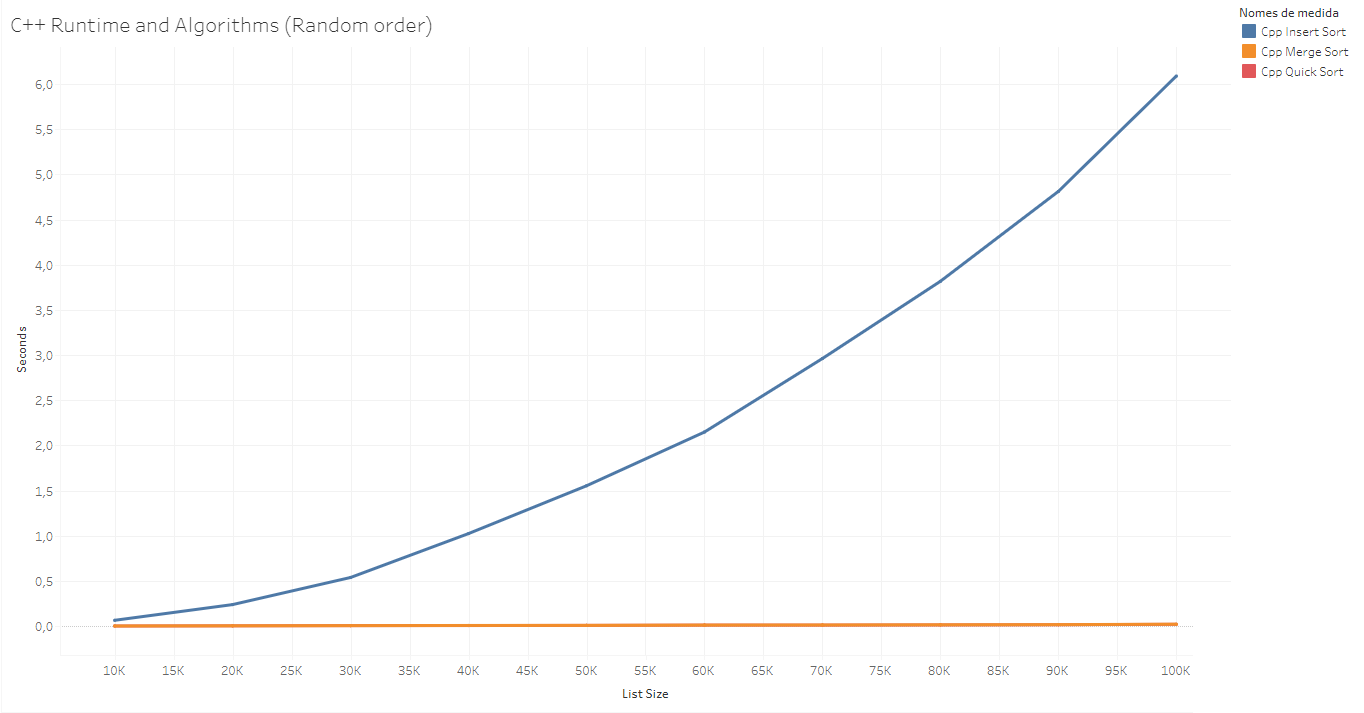
\includegraphics[scale=0.3]{images/runtime_cppONLY-random.png}
	\end{figure}
	
	\begin{figure}[!h]
		\centering
		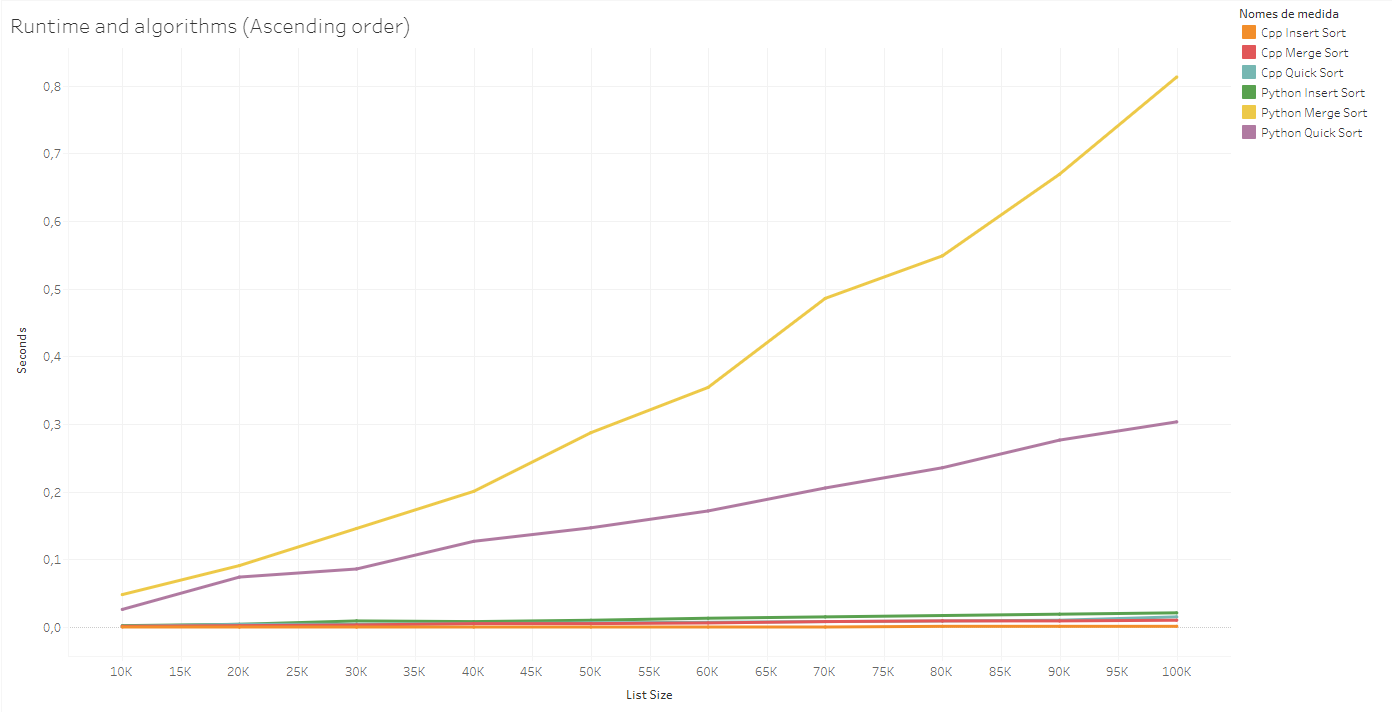
\includegraphics[scale=0.3]{images/runtime_ALL-ascending.png}
		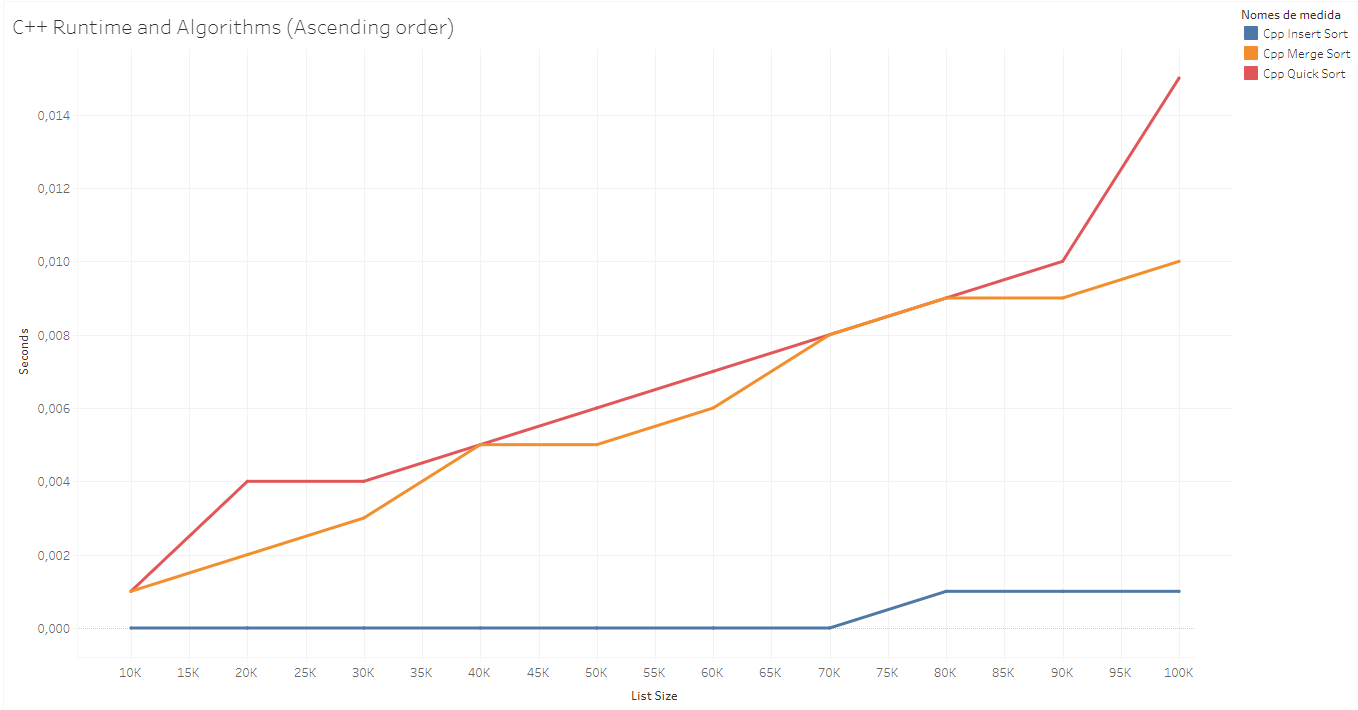
\includegraphics[scale=0.3]{images/runtime_cppONLY-ascending.png}		
	\end{figure}
	
	\begin{figure}[!h]
		\centering
		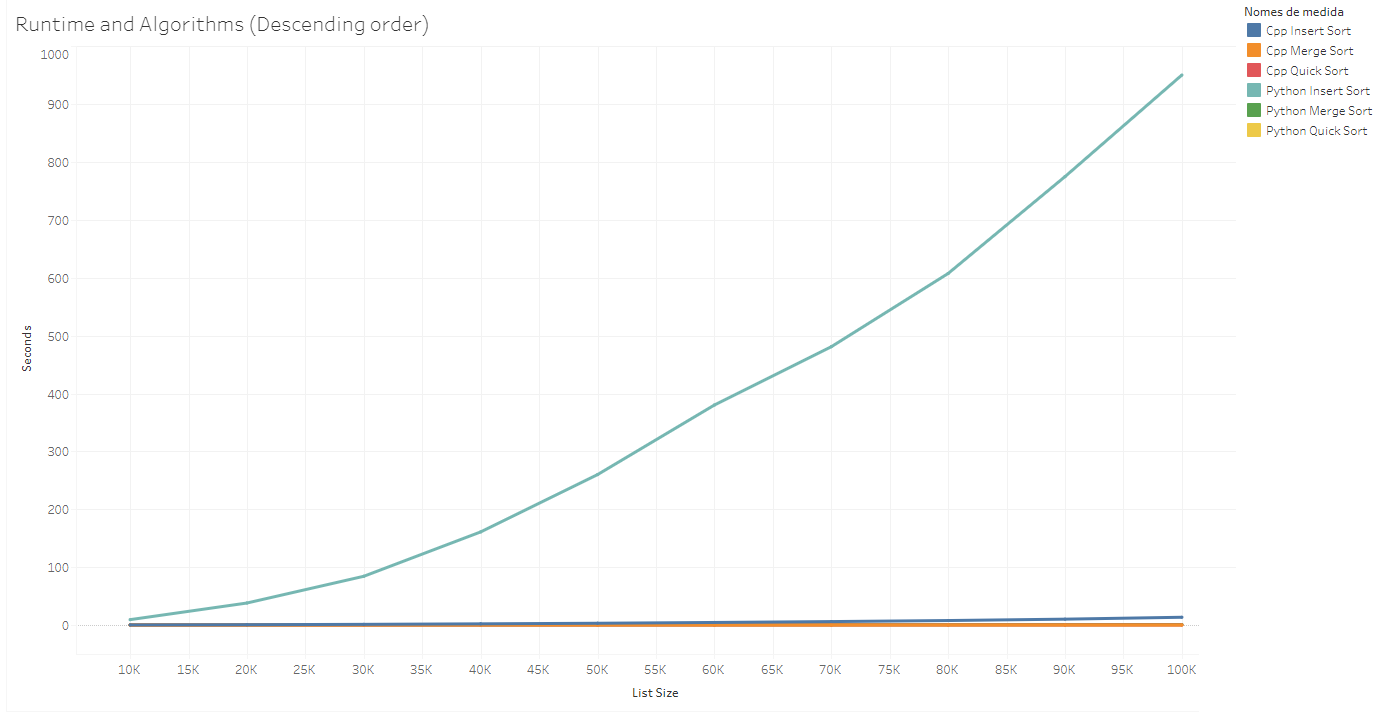
\includegraphics[scale=0.3]{images/runtime_ALL-descending.png}
		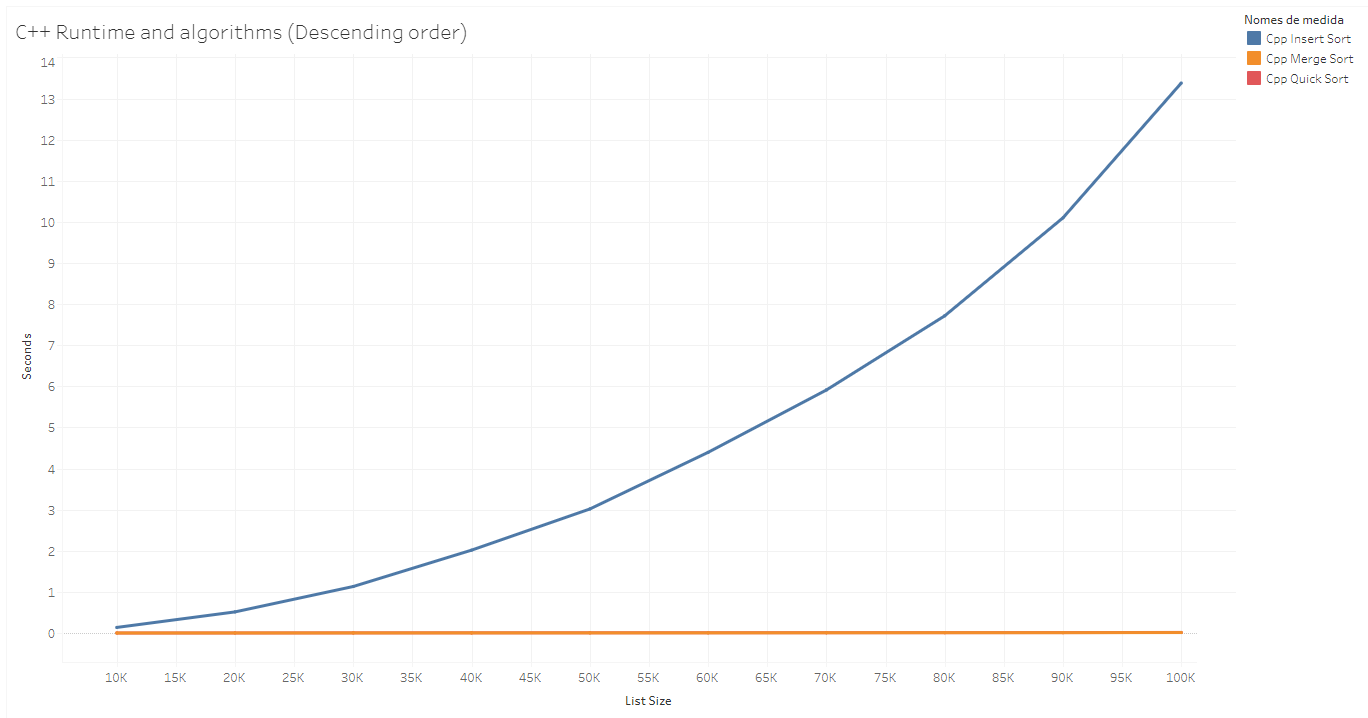
\includegraphics[scale=0.3]{images/runtime_cppONLY-descending.png}
	\end{figure}
	
\end{document}